%!TeX root=../gardentop.tex
\chapter{In the Garden} 
	
\begin{figure}[t!]
\centering

\includegraphics[width=\linewidth]{august}
\end{figure}

 \lettrine[]{I}{n} each century since the beginning of the world wonderful things have been discovered. In the last century more amazing things were found out than in any century before. In this new century hundreds of things still more astounding will be brought to light. At first people refuse to believe that a strange new thing can be done, then they begin to hope it can be done, then they see it can be done—then it is done and all the world wonders why it was not done centuries ago. One of the new things people began to find out in the last century was that thoughts—just mere thoughts—are as powerful as electric batteries—as good for one as sunlight is, or as bad for one as poison. To let a sad thought or a bad one get into your mind is as dangerous as letting a scarlet fever germ get into your body. If you let it stay there after it has got in you may never get over it as long as you live.

So long as Mistress Mary's mind was full of disagreeable thoughts about her dislikes and sour opinions of people and her determination not to be pleased by or interested in anything, she was a yellow-faced, sickly, bored and wretched child. Circumstances, however, were very kind to her, though she was not at all aware of it. They began to push her about for her own good. When her mind gradually filled itself with robins, and moorland cottages crowded with children, with queer crabbed old gardeners and common little Yorkshire housemaids, with springtime and with secret gardens coming alive day by day, and also with a moor boy and his <creatures,> there was no room left for the disagreeable thoughts which affected her liver and her digestion and made her yellow and tired.

So long as Colin shut himself up in his room and thought only of his fears and weakness and his detestation of people who looked at him and reflected hourly on humps and early death, he was a hysterical half-crazy little hypochondriac who knew nothing of the sunshine and the spring and also did not know that he could get well and could stand upon his feet if he tried to do it. When new beautiful thoughts began to push out the old hideous ones, life began to come back to him, his blood ran healthily through his veins and strength poured into him like a flood. His scientific experiment was quite practical and simple and there was nothing weird about it at all. Much more surprising things can happen to any one who, when a disagreeable or discouraged thought comes into his mind, just has the sense to remember in time and push it out by putting in an agreeable determinedly courageous one. Two things cannot be in one place.

\begin{verse}
<Where you tend a rose, my lad,\\
A thistle cannot grow.>
\end{verse}

While the secret garden was coming alive and two children were coming alive with it, there was a man wandering about certain far-away beautiful places in the Norwegian fiords and the valleys and mountains of Switzerland and he was a man who for ten years had kept his mind filled with dark and heart-broken thinking. He had not been courageous; he had never tried to put any other thoughts in the place of the dark ones. He had wandered by blue lakes and thought them; he had lain on mountain-sides with sheets of deep blue gentians blooming all about him and flower breaths filling all the air and he had thought them. A terrible sorrow had fallen upon him when he had been happy and he had let his soul fill itself with blackness and had refused obstinately to allow any rift of light to pierce through. He had forgotten and deserted his home and his duties. When he traveled about, darkness so brooded over him that the sight of him was a wrong done to other people because it was as if he poisoned the air about him with gloom. Most strangers thought he must be either half mad or a man with some hidden crime on his soul. He was a tall man with a drawn face and crooked shoulders and the name he always entered on hotel registers was, <Archibald Craven, Misselthwaite Manor, Yorkshire, England.>

He had traveled far and wide since the day he saw Mistress Mary in his study and told her she might have her <bit of earth.> He had been in the most beautiful places in Europe, though he had remained nowhere more than a few days. He had chosen the quietest and remotest spots. He had been on the tops of mountains whose heads were in the clouds and had looked down on other mountains when the sun rose and touched them with such light as made it seem as if the world were just being born.

But the light had never seemed to touch himself until one day when he realized that for the first time in ten years a strange thing had happened. He was in a wonderful valley in the Austrian Tyrol and he had been walking alone through such beauty as might have lifted any man's soul out of shadow. He had walked a long way and it had not lifted his. But at last he had felt tired and had thrown himself down to rest on a carpet of moss by a stream. It was a clear little stream which ran quite merrily along on its narrow way through the luscious damp greenness. Sometimes it made a sound rather like very low laughter as it bubbled over and round stones. He saw birds come and dip their heads to drink in it and then flick their wings and fly away. It seemed like a thing alive and yet its tiny voice made the stillness seem deeper. The valley was very, very still.

As he sat gazing into the clear running of the water, Archibald Craven gradually felt his mind and body both grow quiet, as quiet as the valley itself. He wondered if he were going to sleep, but he was not. He sat and gazed at the sunlit water and his eyes began to see things growing at its edge. There was one lovely mass of blue forget-me-nots growing so close to the stream that its leaves were wet and at these he found himself looking as he remembered he had looked at such things years ago. He was actually thinking tenderly how lovely it was and what wonders of blue its hundreds of little blossoms were. He did not know that just that simple thought was slowly filling his mind—filling and filling it until other things were softly pushed aside. It was as if a sweet clear spring had begun to rise in a stagnant pool and had risen and risen until at last it swept the dark water away. But of course he did not think of this himself. He only knew that the valley seemed to grow quieter and quieter as he sat and stared at the bright delicate blueness. He did not know how long he sat there or what was happening to him, but at last he moved as if he were awakening and he got up slowly and stood on the moss carpet, drawing a long, deep, soft breath and wondering at himself. Something seemed to have been unbound and released in him, very quietly.

<What is it?> he said, almost in a whisper, and he passed his hand over his forehead. <I almost feel as if—I were alive!>

I do not know enough about the wonderfulness of undiscovered things to be able to explain how this had happened to him. Neither does any one else yet. He did not understand at all himself—but he remembered this strange hour months afterward when he was at Misselthwaite again and he found out quite by accident that on this very day Colin had cried out as he went into the secret garden:

<I am going to live forever and ever and ever!>

The singular calmness remained with him the rest of the evening and he slept a new reposeful sleep; but it was not with him very long. He did not know that it could be kept. By the next night he had opened the doors wide to his dark thoughts and they had come trooping and rushing back. He left the valley and went on his wandering way again. But, strange as it seemed to him, there were minutes—sometimes half-hours—when, without his knowing why, the black burden seemed to lift itself again and he knew he was a living man and not a dead one. Slowly—slowly—for no reason that he knew of—he was <coming alive> with the garden.

As the golden summer changed into the deeper golden autumn he went to the Lake of Como. There he found the loveliness of a dream. He spent his days upon the crystal blueness of the lake or he walked back into the soft thick verdure of the hills and tramped until he was tired so that he might sleep. But by this time he had begun to sleep better, he knew, and his dreams had ceased to be a terror to him.

<Perhaps,> he thought, <my body is growing stronger.>

It was growing stronger but—because of the rare peaceful hours when his thoughts were changed—his soul was slowly growing stronger, too. He began to think of Misselthwaite and wonder if he should not go home. Now and then he wondered vaguely about his boy and asked himself what he should feel when he went and stood by the carved four-posted bed again and looked down at the sharply chiseled ivory-white face while it slept and the black lashes rimmed so startlingly the close-shut eyes. He shrank from it.

One marvel of a day he had walked so far that when he returned the moon was high and full and all the world was purple shadow and silver. The stillness of lake and shore and wood was so wonderful that he did not go into the villa he lived in. He walked down to a little bowered terrace at the water's edge and sat upon a seat and breathed in all the heavenly scents of the night. He felt the strange calmness stealing over him and it grew deeper and deeper until he fell asleep.

He did not know when he fell asleep and when he began to dream; his dream was so real that he did not feel as if he were dreaming. He remembered afterward how intensely wide awake and alert he had thought he was. He thought that as he sat and breathed in the scent of the late roses and listened to the lapping of the water at his feet he heard a voice calling. It was sweet and clear and happy and far away. It seemed very far, but he heard it as distinctly as if it had been at his very side.

<Archie! Archie! Archie!> it said, and then again, sweeter and clearer than before, <Archie! Archie!>

He thought he sprang to his feet not even startled. It was such a real voice and it seemed so natural that he should hear it.

<Lilias! Lilias!> he answered. <Lilias! where are you?>

<In the garden,> it came back like a sound from a golden flute. <In the garden!>

And then the dream ended. But he did not awaken. He slept soundly and sweetly all through the lovely night. When he did awake at last it was brilliant morning and a servant was standing staring at him. He was an Italian servant and was accustomed, as all the servants of the villa were, to accepting without question any strange thing his foreign master might do. No one ever knew when he would go out or come in or where he would choose to sleep or if he would roam about the garden or lie in the boat on the lake all night. The man held a salver with some letters on it and he waited quietly until Mr~Craven took them. When he had gone away Mr~Craven sat a few moments holding them in his hand and looking at the lake. His strange calm was still upon him and something more—a lightness as if the cruel thing which had been done had not happened as he thought—as if something had changed. He was remembering the dream—the real—real dream.

<In the garden!> he said, wondering at himself. <In the garden! But the door is locked and the key is buried deep.>

When he glanced at the letters a few minutes later he saw that the one lying at the top of the rest was an English letter and came from Yorkshire. It was directed in a plain woman's hand but it was not a hand he knew. He opened it, scarcely thinking of the writer, but the first words attracted his attention at once.

\begin{quotation}
\noindent Dear Sir:

I am Susan Sowerby that made bold to speak to you once on the moor. It was about Miss Mary I spoke. I will make bold to speak again. Please, sir, I would come home if I was you. I think you would be glad to come and—if you will excuse me, sir—I think your lady would ask you to come if she was here.

\begin{flushright}
Your obedient servant\\
Susan Sowerby.
\end{flushright}
\end{quotation}

Mr~Craven read the letter twice before he put it back in its envelope. He kept thinking about the dream.

<I will go back to Misselthwaite,> he said. <Yes, I'll go at once.>

And he went through the garden to the villa and ordered Pitcher to prepare for his return to England.

In a few days he was in Yorkshire again, and on his long railroad journey he found himself thinking of his boy as he had never thought in all the ten years past. During those years he had only wished to forget him. Now, though he did not intend to think about him, memories of him constantly drifted into his mind. He remembered the black days when he had raved like a madman because the child was alive and the mother was dead. He had refused to see it, and when he had gone to look at it at last it had been such a weak wretched thing that every one had been sure it would die in a few days. But to the surprise of those who took care of it the days passed and it lived and then every one believed it would be a deformed and crippled creature.

He had not meant to be a bad father, but he had not felt like a father at all. He had supplied doctors and nurses and luxuries, but he had shrunk from the mere thought of the boy and had buried himself in his own misery. The first time after a year's absence he returned to Misselthwaite and the small miserable looking thing languidly and indifferently lifted to his face the great gray eyes with black lashes round them, so like and yet so horribly unlike the happy eyes he had adored, he could not bear the sight of them and turned away pale as death. After that he scarcely ever saw him except when he was asleep, and all he knew of him was that he was a confirmed invalid, with a vicious, hysterical, half-insane temper. He could only be kept from furies dangerous to himself by being given his own way in every detail.

All this was not an uplifting thing to recall, but as the train whirled him through mountain passes and golden plains the man who was <coming alive> began to think in a new way and he thought long and steadily and deeply.

<Perhaps I have been all wrong for ten years,> he said to himself. <Ten years is a long time. It may be too late to do anything—quite too late. What have I been thinking of!>

Of course this was the wrong Magic—to begin by saying <too late.> Even Colin could have told him that. But he knew nothing of Magic—either black or white. This he had yet to learn. He wondered if Susan Sowerby had taken courage and written to him only because the motherly creature had realized that the boy was much worse—was fatally ill. If he had not been under the spell of the curious calmness which had taken possession of him he would have been more wretched than ever. But the calm had brought a sort of courage and hope with it. Instead of giving way to thoughts of the worst he actually found he was trying to believe in better things.

<Could it be possible that she sees that I may be able to do him good and control him?> he thought. <I will go and see her on my way to Misselthwaite.>

But when on his way across the moor he stopped the carriage at the cottage, seven or eight children who were playing about gathered in a group and bobbing seven or eight friendly and polite curtsies told him that their mother had gone to the other side of the moor early in the morning to help a woman who had a new baby. <Our Dickon,> they volunteered, was over at the Manor working in one of the gardens where he went several days each week.

Mr~Craven looked over the collection of sturdy little bodies and round red-cheeked faces, each one grinning in its own particular way, and he awoke to the fact that they were a healthy likable lot. He smiled at their friendly grins and took a golden sovereign from his pocket and gave it to <our 'Lizabeth Ellen> who was the oldest.

<If you divide that into eight parts there will be half a crown for each of you,> he said.

Then amid grins and chuckles and bobbing of curtsies he drove away, leaving ecstasy and nudging elbows and little jumps of joy behind.

The drive across the wonderfulness of the moor was a soothing thing. Why did it seem to give him a sense of home-coming which he had been sure he could never feel again—that sense of the beauty of land and sky and purple bloom of distance and a warming of the heart at drawing nearer to the great old house which had held those of his blood for six hundred years? How he had driven away from it the last time, shuddering to think of its closed rooms and the boy lying in the four-posted bed with the brocaded hangings. Was it possible that perhaps he might find him changed a little for the better and that he might overcome his shrinking from him? How real that dream had been—how wonderful and clear the voice which called back to him, <In the garden—In the garden!>

<I will try to find the key,> he said. <I will try to open the door. I must—though I don't know why.>

When he arrived at the Manor the servants who received him with the usual ceremony noticed that he looked better and that he did not go to the remote rooms where he usually lived attended by Pitcher. He went into the library and sent for Mrs~Medlock. She came to him somewhat excited and curious and flustered.

<How is Master Colin, Medlock?> he inquired.

<Well, sir,> Mrs~Medlock answered, <he's—he's different, in a manner of speaking.>

<Worse?> he suggested.

Mrs~Medlock really was flushed.

<Well, you see, sir,> she tried to explain, <neither Dr~Craven, nor the nurse, nor me can exactly make him out.>

<Why is that?>

<To tell the truth, sir, Master Colin might be better and he might be changing for the worse. His appetite, sir, is past understanding—and his ways—>

<Has he become more—more peculiar?> her master asked, knitting his brows anxiously.

<That's it, sir. He's growing very peculiar—when you compare him with what he used to be. He used to eat nothing and then suddenly he began to eat something enormous—and then he stopped again all at once and the meals were sent back just as they used to be. You never knew, sir, perhaps, that out of doors he never would let himself be taken. The things we've gone through to get him to go out in his chair would leave a body trembling like a leaf. He'd throw himself into such a state that Dr~Craven said he couldn't be responsible for forcing him. Well, sir, just without warning—not long after one of his worst tantrums he suddenly insisted on being taken out every day by Miss Mary and Susan Sowerby's boy Dickon that could push his chair. He took a fancy to both Miss Mary and Dickon, and Dickon brought his tame animals, and, if you'll credit it, sir, out of doors he will stay from morning until night.>

<How does he look?> was the next question.

<If he took his food natural, sir, you'd think he was putting on flesh—but we're afraid it may be a sort of bloat. He laughs sometimes in a queer way when he's alone with Miss Mary. He never used to laugh at all. Dr~Craven is coming to see you at once, if you'll allow him. He never was as puzzled in his life.>

<Where is Master Colin now?> Mr~Craven asked.

<In the garden, sir. He's always in the garden—though not a human creature is allowed to go near for fear they'll look at him.>

Mr~Craven scarcely heard her last words.

<In the garden,> he said, and after he had sent Mrs~Medlock away he stood and repeated it again and again. <In the garden!>

He had to make an effort to bring himself back to the place he was standing in and when he felt he was on earth again he turned and went out of the room. He took his way, as Mary had done, through the door in the shrubbery and among the laurels and the fountain beds. The fountain was playing now and was encircled by beds of brilliant autumn flowers. He crossed the lawn and turned into the Long Walk by the ivied walls. He did not walk quickly, but slowly, and his eyes were on the path. He felt as if he were being drawn back to the place he had so long forsaken, and he did not know why. As he drew near to it his step became still more slow. He knew where the door was even though the ivy hung thick over it—but he did not know exactly where it lay—that buried key.

So he stopped and stood still, looking about him, and almost the moment after he had paused he started and listened—asking himself if he were walking in a dream.

The ivy hung thick over the door, the key was buried under the shrubs, no human being had passed that portal for ten lonely years—and yet inside the garden there were sounds. They were the sounds of running scuffling feet seeming to chase round and round under the trees, they were strange sounds of lowered suppressed voices—exclamations and smothered joyous cries. It seemed actually like the laughter of young things, the uncontrollable laughter of children who were trying not to be heard but who in a moment or so—as their excitement mounted—would burst forth. What in heaven's name was he dreaming of—what in heaven's name did he hear? Was he losing his reason and thinking he heard things which were not for human ears? Was it that the far clear voice had meant?

And then the moment came, the uncontrollable moment when the sounds forgot to hush themselves. The feet ran faster and faster—they were nearing the garden door—there was quick strong young breathing and a wild outbreak of laughing shouts which could not be contained—and the door in the wall was flung wide open, the sheet of ivy swinging back, and a boy burst through it at full speed and, without seeing the outsider, dashed almost into his arms.

Mr~Craven had extended them just in time to save him from falling as a result of his unseeing dash against him, and when he held him away to look at him in amazement at his being there he truly gasped for breath.

He was a tall boy and a handsome one. He was glowing with life and his running had sent splendid colour leaping to his face. He threw the thick hair back from his forehead and lifted a pair of strange gray eyes—eyes full of boyish laughter and rimmed with black lashes like a fringe. It was the eyes which made Mr~Craven gasp for breath.

<Who—What? Who!> he stammered.

This was not what Colin had expected—this was not what he had planned. He had never thought of such a meeting. And yet to come dashing out—winning a race—perhaps it was even better. He drew himself up to his very tallest. Mary, who had been running with him and had dashed through the door too, believed that he managed to make himself look taller than he had ever looked before—inches taller.

<Father,> he said, <I'm Colin. You can't believe it. I scarcely can myself. I'm Colin.>

Like Mrs~Medlock, he did not understand what his father meant when he said hurriedly:

<In the garden! In the garden!>

<Yes,> hurried on Colin. <It was the garden that did it—and Mary and Dickon and the creatures—and the Magic. No one knows. We kept it to tell you when you came. I'm well, I can beat Mary in a race. I'm going to be an athlete.>

He said it all so like a healthy boy—his face flushed, his words tumbling over each other in his eagerness—that Mr~Craven's soul shook with unbelieving joy.

Colin put out his hand and laid it on his father's arm.

<Aren't you glad, Father?> he ended.

<Aren't you glad? I'm going to live forever and ever and ever!>

Mr~Craven put his hands on both the boy's shoulders and held him still. He knew he dared not even try to speak for a moment.

<Take me into the garden, my boy,> he said at last. <And tell me all about it.>

And so they led him in.

The place was a wilderness of autumn gold and purple and violet blue and flaming scarlet and on every side were sheaves of late lilies standing together—lilies which were white or white and ruby. He remembered well when the first of them had been planted that just at this season of the year their late glories should reveal themselves. Late roses climbed and hung and clustered and the sunshine deepening the hue of the yellowing trees made one feel that one stood in an embowered temple of gold. The newcomer stood silent just as the children had done when they came into its grayness. He looked round and round.

<I thought it would be dead,> he said.

<Mary thought so at first,> said Colin. <But it came alive.>

Then they sat down under their tree—all but Colin, who wanted to stand while he told the story.

It was the strangest thing he had ever heard, Archibald Craven thought, as it was poured forth in headlong boy fashion. Mystery and Magic and wild creatures, the weird midnight meeting—the coming of the spring—the passion of insulted pride which had dragged the young Rajah to his feet to defy old Ben Weatherstaff to his face. The odd companionship, the play acting, the great secret so carefully kept. The listener laughed until tears came into his eyes and sometimes tears came into his eyes when he was not laughing. The Athlete, the Lecturer, the Scientific Discoverer was a laughable, lovable, healthy young human thing.

<Now,> he said at the end of the story, <it need not be a secret any more. I dare say it will frighten them nearly into fits when they see me—but I am never going to get into the chair again. I shall walk back with you, Father—to the house.>

Ben Weatherstaff's duties rarely took him away from the gardens, but on this occasion he made an excuse to carry some vegetables to the kitchen and being invited into the servants' hall by Mrs~Medlock to drink a glass of beer he was on the spot—as he had hoped to be—when the most dramatic event Misselthwaite Manor had seen during the present generation actually took place.

One of the windows looking upon the courtyard gave also a glimpse of the lawn. Mrs~Medlock, knowing Ben had come from the gardens, hoped that he might have caught sight of his master and even by chance of his meeting with Master Colin.

<Did you see either of them, Weatherstaff?> she asked.

Ben took his beer-mug from his mouth and wiped his lips with the back of his hand.

<Aye, that I did,> he answered with a shrewdly significant air.

<Both of them?> suggested Mrs~Medlock.

<Both of 'em,> returned Ben Weatherstaff. <Thank ye kindly, ma'am, I could sup up another mug of it.>

<Together?> said Mrs~Medlock, hastily overfilling his beer-mug in her excitement.

<Together, ma'am,> and Ben gulped down half of his new mug at one gulp.

<Where was Master Colin? How did he look? What did they say to each other?>

<I didna' hear that,> said Ben, <along o' only bein' on th' step-ladder lookin' over th' wall. But I'll tell thee this. There's been things goin' on outside as you house people knows nowt about. An' what tha'll find out tha'll find out soon.>

And it was not two minutes before he swallowed the last of his beer and waved his mug solemnly toward the window which took in through the shrubbery a piece of the lawn.

<Look there,> he said, <if tha's curious. Look what's comin' across th' grass.>

When Mrs~Medlock looked she threw up her hands and gave a little shriek and every man and woman servant within hearing bolted across the servants' hall and stood looking through the window with their eyes almost starting out of their heads.

Across the lawn came the Master of Misselthwaite and he looked as many of them had never seen him. And by his side with his head up in the air and his eyes full of laughter walked as strongly and steadily as any boy in Yorkshire—Master Colin!


\begin{a4}
	\begin{tikzpicture}[remember picture, overlay]  
		\node (theend) at ($(current page.south)+(0cm,4.25cm)$) {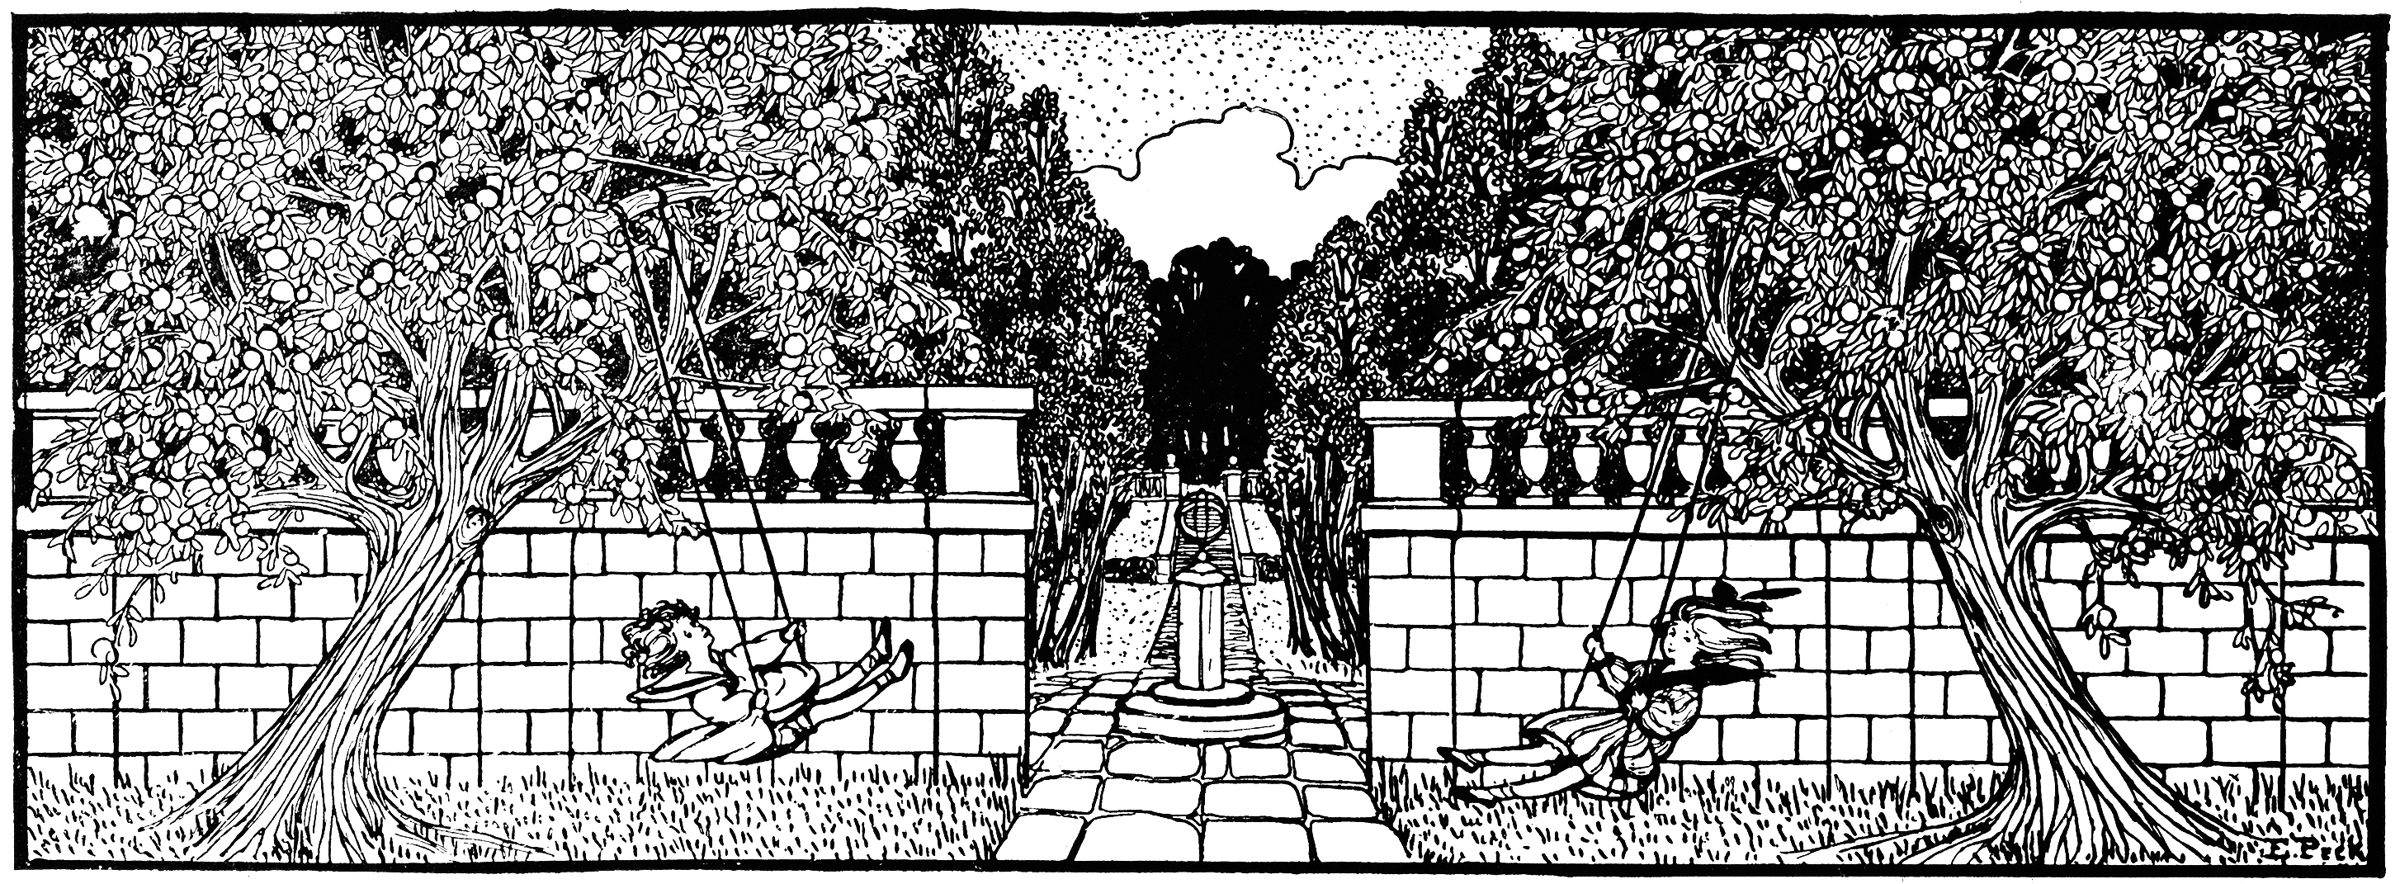
\includegraphics[width=1.05\textwidth]{garden}};
	\end{tikzpicture}
	

\end{a4}

\begin{letter}
	\pagenumbering{gobble} %since it's the last page, no need to restore things
	\begin{tikzpicture}[remember picture, overlay]  
		\node (theend) at ($(current page.south)+(0cm,3cm)$) {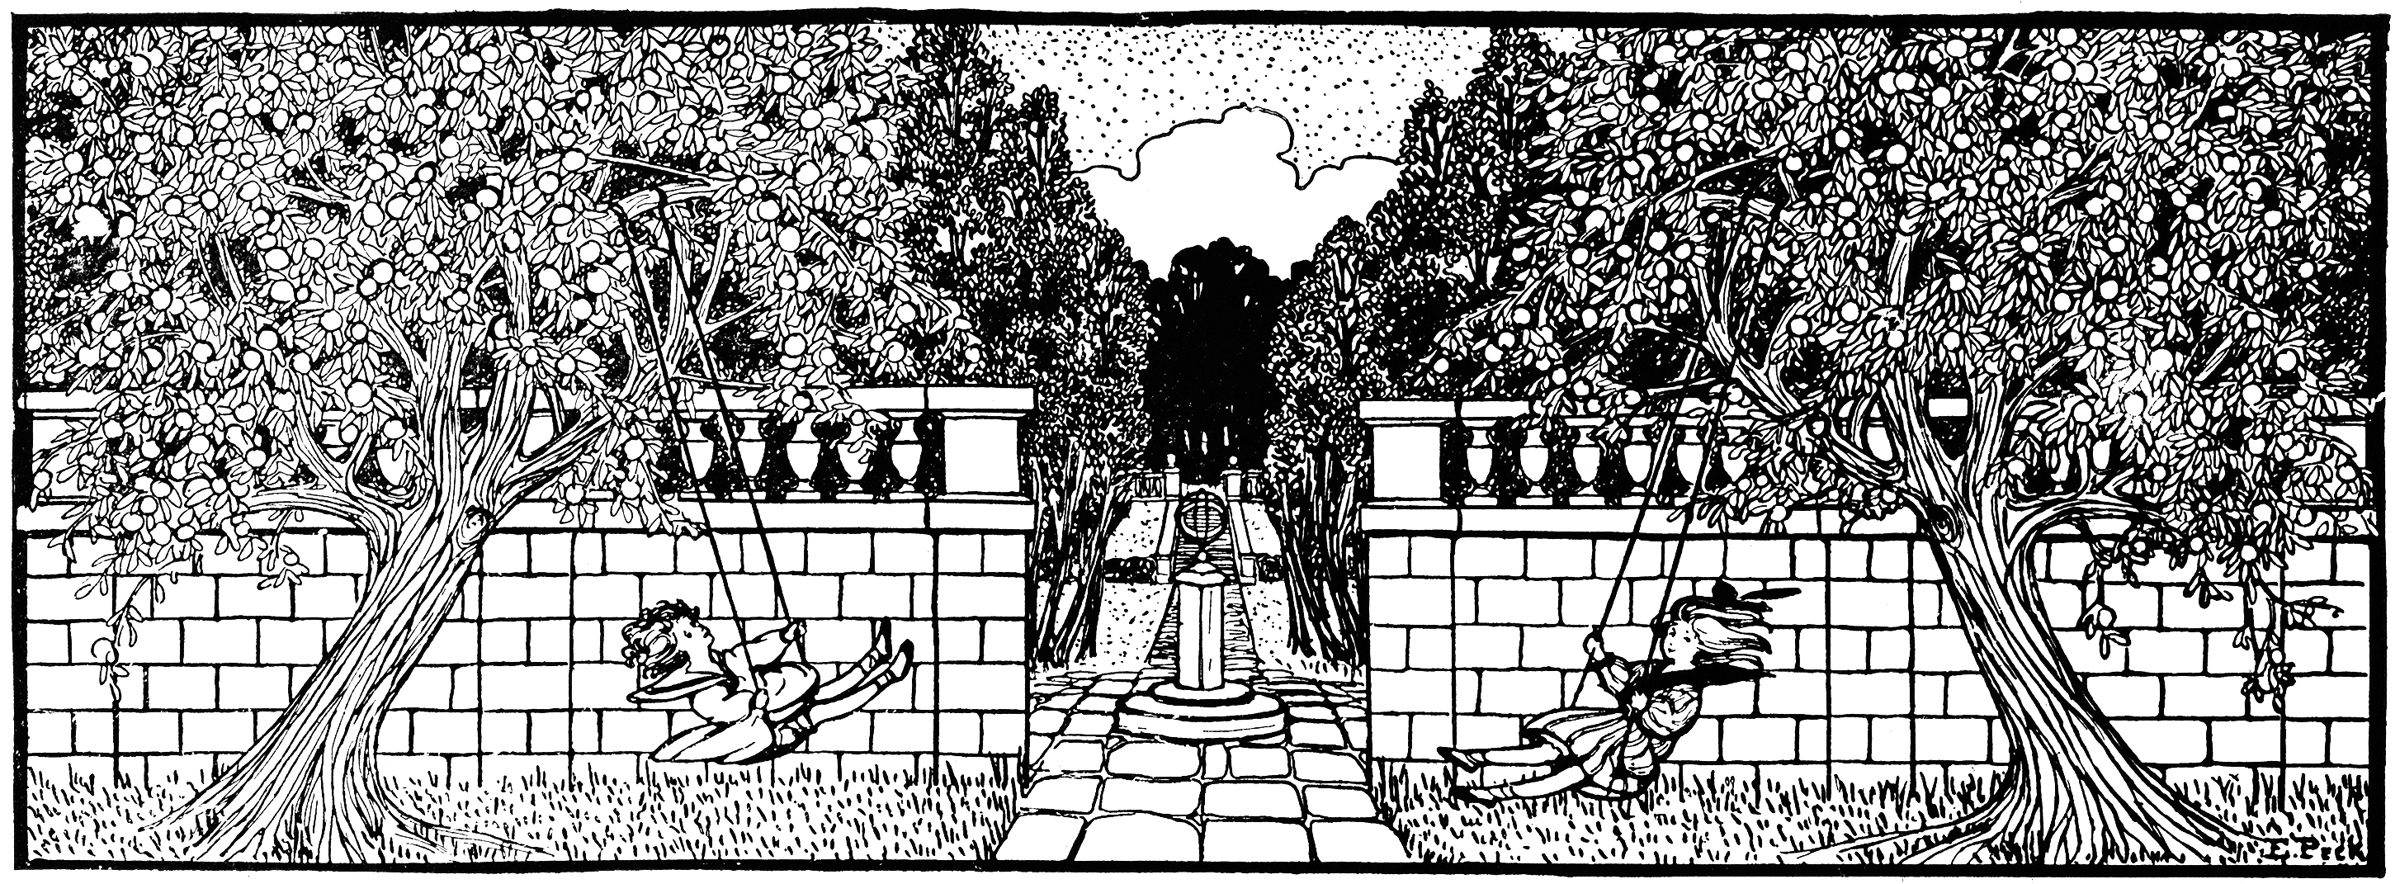
\includegraphics[width=.9\textwidth]{garden}};
	\end{tikzpicture}
\end{letter}